\documentclass[a4paper]{oblivoir}
\usepackage{amsmath,amssymb,kotex,mdframed,paralist,tabu}
\usepackage{fapapersize}
\usefapapersize{210mm,297mm,20mm,*,20mm,*}

\usepackage{tabto,pifont}
\TabPositions{0.2\textwidth,0.4\textwidth,0.6\textwidth,0.8\textwidth}

%%% 객관식 선지
\newcommand\one{\ding{172}}
\newcommand\two{\ding{173}}
\newcommand\three{\ding{174}}
\newcommand\four{\ding{175}}
\newcommand\five{\ding{176}}
\usepackage{tabto,pifont}
%\TabPositions{0.2\textwidth,0.4\textwidth,0.6\textwidth,0.8\textwidth}

\newcommand\taba[5]{\par\noindent
\one\:{#1}
\tabto{0.2\textwidth}\two\:\:{#2}
\tabto{0.4\textwidth}\three\:\:{#3}
\tabto{0.6\textwidth}\four\:\:{#4}
\tabto{0.8\textwidth}\five\:\:{#5}}

\newcommand\tabb[5]{\par\noindent
\one\:{#1}
\tabto{0.33\textwidth}\two\:\:{#2}
\tabto{0.67\textwidth}\three\:\:{#3}\medskip\par\noindent
\four\:\:{#4}
\tabto{0.33\textwidth}\five\:\:{#5}}

\newcommand\tabc[5]{\par\noindent
\one\:{#1}
\tabto{0.5\textwidth}\two\:\:{#2}\medskip\par\noindent
\three\:\:{#3}
\tabto{0.5\textwidth}\four\:\:{#4}\medskip\par\noindent
\five\:\:{#5}}

\newcommand\tabd[5]{\par\noindent
\one\:{#1}\medskip\par\noindent
\two\:\:{#2}\medskip\par\noindent
\three\:\:{#3}\medskip\par\noindent
\four\:\:{#4}\medskip\par\noindent
\five\:\:{#5}}

\newcommand\vs[1]{\par\vspace{30pt}}

\usepackage{graphicx}

%\pagestyle{empty}

%%% Counters
\newcounter{num}

%%% Commands
\newcommand{\prob}[1]
{\bigskip\bigskip\noindent\refstepcounter{num}\textbf{문제 \arabic{num})} #1\par\noindent}

\newcommand\pb[1]{\ensuremath{\fbox{\phantom{#1}}}}

\newcommand\ba{\ensuremath{\:|\:}}

\newcommand\an[1]{\bigskip\par\noindent\textbf{문제 #1)}\par\noindent}

%%% Meta Commands
\let\oldsection\section
\renewcommand\section{\clearpage\oldsection}

\let\emph\textsf

\begin{document}
\begin{center}
\LARGE태희, 미니테스트 10
\end{center}
\begin{flushright}
날짜 : 2018년 \(\pb3\)월 \(\pb{10}\)일 \(\pb{월}\)요일
,\qquad
제한시간 : \pb{17년}분
,\qquad
점수 : \pb{20} / \pb{20}
\end{flushright}

%
\prob{다음 <보기>에서 옳은 것만을 있는 대로 고른 것은?}
\begin{mdframed}[frametitle=<보기>]
\begin{enumerate}
\item[ㄱ.]
실수 \(a\), \(b\)에 대하여 \(|a+b|+|a-b|\ge|2b|\)
\item[ㄴ.]
실수 \(x\), \(y\)에 대하여 \(x^2-3xy-y^2\ge xy-4y^2\)
\item[ㄷ.]
실수 \(x\), \(y\)에 대하여 \(5\sqrt{x^2+y^2}\ge 3x-4y\)
\end{enumerate}
\end{mdframed}
\tabb{\text{ㄱ}}{\text{ㄷ}}{\text{ㄱ, ㄷ}}{\text{ㄴ, ㄷ}}{\text{ㄱ, ㄴ, ㄷ}}
\vs

%
\prob{\(x>0\), \(y>0\)이고 \(x+3y=6\)일 때, \(\sqrt{x}+\sqrt{3y}\)의 최댓값을 구하여라.}
\taba{\(\sqrt{10}\)}{\(2\sqrt3\)}{\(\sqrt{14}\)}4{3\(\sqrt2\)}
\vs

%
\prob{실수 \(a\), \(b\)에 대하여 \(a^2+b^2=4\)일 때, \(a^2+5a+b^2+4b\)의 최댓값을 구하시오.}
%\taba{\(2\sqrt{41}+2\)}{\(2\sqrt{41}+2\)}{\(2\sqrt{41}+2\)}{\(2\sqrt{41}+2\)}{\(2\sqrt{41}+2\)}
\vs

%
\prob{실수 전체에서 정의된 함수}
\[f(x)=
\begin{cases}
-x+3		&(x\ge1)\\
ax+b 	&(x<1)
\end{cases}\]
가 일대일 대응일 때, 상수 \(b\)의 값의 범위를 구하여라.
\taba{\(b<2\)}{\(b<3\)}{\(b<4\)}{\(b>2\)}{\(b>3\)}
\vs

%
\prob{두 집합 \(X=\{x\ba x\ge4\}\), \(Y=\{y\ba y\ge3\}\)에 대하여 \(X\)에서 \(Y\)로의 함수 \(f(x)=2^x+(k-10)\) 일대일대응일 때, 상수 \(a\)의 값을 구하여라.}
\taba{\(-5\)}{\(-4\)}{\(-3\)}{\(-2\)}{\(-1\)}
\vs

\prob{유리함수 \(y=\frac{bx+c}{x+a}\)의 그래프가 점 \((2,6)\)을 지나고 점근선의 방정식이 \(x=3\), \(y=2\)일 때, \(a+b+c\)의 값을 구하여라.}
\taba{\(-11\)}{\(-7\)}{\(3\)}15

%
\prob{유리함수 \(y=\frac{2x+1}{x-1}\)의 그래프가 두 직선 \(y=x+a\), \(y=-x+b\)에 대하여 대칭일 때, \(a+b\)의 값을 구하여라.}
\taba12345
\vs

%
\prob{유리함수 \(y=\frac{2x-1}{x-1}\)의 그래프와 직선 \(y=kx+2\)가 만나지 않도록 하는 실수 \(k\)의 값의 범위를 구하여라.}
\vs

%
\prob{두 함수 \(y=\sqrt{2x+1}\), \(y=x+k\)의 그래프가 서로 다른 두 점에서 만날 때, 실수 \(k\)의 값의 범위는?}
\taba{\(k\ge1\)}{\(k<1\)}{\(k>\frac12\)}{\(\frac12<k\le1\)}{\(\frac12\le k<1\)}
\vs

\noindent\begin{minipage}{.6\textwidth}
%
\prob{무리함수 \(y=-\sqrt{ax+b}+c\)의 그래프가 아래 그림과 같을 떄, \(a+b+c\)의 값을 구하여라.}
\end{minipage}
\begin{minipage}{.4\textwidth}
\centering
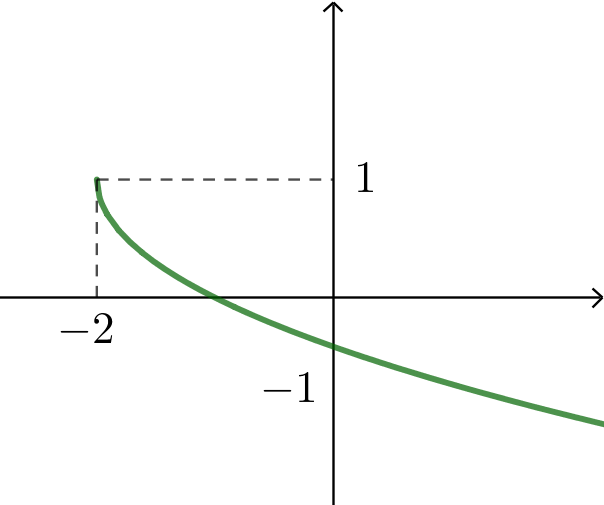
\includegraphics[width=.5\textwidth]{irrational}
\end{minipage}
\taba6789{10}
\vs

%
\prob{함수 \(y=\sqrt{2x-1}\)의 그래프와 함수 \(y=\sqrt{5-x}+k\)의 그래프와 만나도록 하는 실수 \(k\)의 최댓값을 구하시오.}
\vs

%
\prob{다음 지수방정식을 풀어라.}
\begin{enumerate}[(1)]
\item
\(2^{2x}-3\cdot2^x-4=0\)
\item
\(2^x+2^{-x}=2\)
\item
\(\begin{cases}
2^x+3^y=17\\
2^{x+1}-3^y=7
\end{cases}\)
\end{enumerate}
\end{document}